\documentclass[a4paper]{article}
\usepackage[utf8]{inputenc}
\usepackage[T1]{fontenc}
\usepackage[ngerman]{babel}
\usepackage{graphicx}
\usepackage{tikz}
\usepackage{amsmath}
\usepackage{siunitx}
\sisetup{
	locale = DE,
	separate-uncertainty,
	range-units = brackets,
	list-units = single,
	per-mode=symbol-or-fraction
}
\usepackage{hyperref}
\usepackage{caption}

% Autor: Michael Krause
% E-Mail: m_krause@posteo.de

% Lizenzhinweis
% Dieses Dokument ist unter der License: CC BY-SA 4.0 Lizenz veröffentlicht. 
% Die Bedingungen der Lizenz finden Sie unter creativecommons.org/licenses/by-sa/4.0/


% Konfiguration des Seitenlayouts
\usepackage[a4paper, landscape, margin=1cm]{geometry}

\begin{document}
	\pagestyle{empty}   % Keine Seitennummern auf allen Seiten
	
	% Kein extra Raum am Anfang von Paragraphen
	\setlength{\parindent}{0pt}
	\setlength{\parskip}{1em} % Etwas Abstand zwischen den Paragraphen
	
	% Einführungstext
	\textbf{CMOS-Technik:} Traditionell werden hochintegrierte Schaltkreise (ICs) heute in einer Transistorschaltungstechnik hergestellt, die weltweit als CMOS-Technik bekannt ist. 
	%Obwohl es seit 2016 vonseiten der IEEE in der „IRDS Roadmap“ Bestrebungen gibt, neue Technologien zu erforschen, können Sie meist sicher sein, dass in Ihren heutigen digital-elektronischen Geräten genau diese Technologie zum Einsatz kommt. 
	CMOS steht dabei für „Complementary Metal-Oxide-Semiconductor“ und versucht, in diesem Namen zu verdeutlichen, wie die Transistoren verschaltet werden und welche Art von Transistoren zum Einsatz kommt.
	Bei Metal-Oxide-Semiconductor (MOS) handelt es sich um eine unipolare Transistorart, die vereinfacht als spannungsgesteuerter Widerstand betrachtet werden kann, welcher drei Anschlüsse besitzt: Gate (1), Drain (2) und Source (3). In digitalen CMOS-Schaltungen arbeiten diese Transistoren als schnelle Schalter, die durch das Gate-Signal vollständig ein oder ausgeschaltet werden. Beim einschalten über das Gate wird eine fast widerstandslose Verbindung zwischen Drain und Source realisiert. Das C in CMOS steht dabei für „Complementary“ und deutet an, dass neben dem p-dotierten MOS-Transistor (PMOS) immer auch sein komplementärer Gegenspieler, der n-dotierte MOS-Transistor (NMOS), zum Einsatz kommt. Dies führt dazu, dass (außer bei Umschaltvorgängen) kein nennenswerter Strom fließt, da entweder der PMOS oder der NMOS Transistor sperrt. PMOS schaltet bei negativer Spannung am Gate und NMOS bei Positiver in Bezug zum Source Anschluss.
 
	\vspace{0.2cm} % Vertikaler Abstand
	
	\noindent % Verhindert Einrückung am Anfang des Absatzes
	\begin{minipage}[b]{0.45\textwidth}
		\centering
		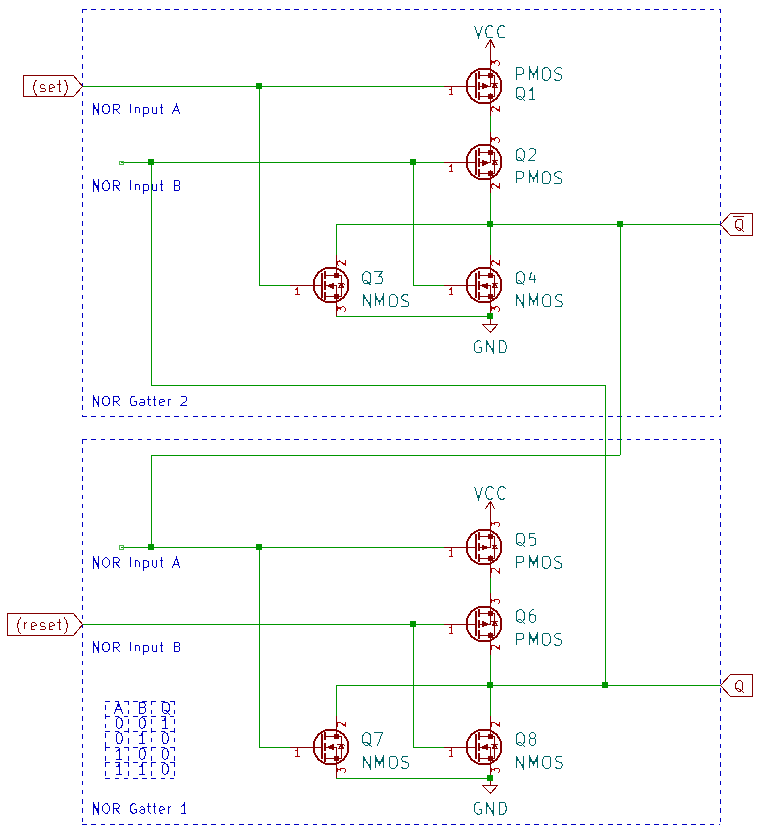
\includegraphics[scale=0.45]{Figures/RS_Latch_Schematic}
	\end{minipage}\hfill % Fügt horizontalen Zwischenraum ein
	\begin{minipage}[b]{0.5\textwidth}
		\centering
		% Text über der Grafik
		\begin{minipage}[t]{\textwidth}
			\centering
			\textbf{Exponat:} Hier haben Sie die Möglichkeit, eine CMOS-Schaltung zu betrachten und zu testen. (siehe links Schaltplan und unten die Realisierung)
			Normalerweise sind derartige CMOS-Transistoren extrem klein (<= 20nm). Um die Verschaltung sichtbar zu machen, wurden hier 8 MOS-Leistungstransistoren in Form eines 1-Bit-Speichers komplementär verschaltet. Interessant ist, dass diese Schaltung aus 2 NOR-Gattern besteht, die normalerweise keine Speicherfunktionalität haben. Durch eine Feedbackverschaltung werden sie jedoch zu einem Speicher umfunktioniert. Auf diese Weise bekommen Sie eine Idee, wie ein statischer RAM funktioniert. 
		\end{minipage}
		% Abstand zwischen Text und Grafik
		\vspace{0.4cm}
		
		\begin{minipage}[b]{\textwidth}
			\centering
			\begin{tikzpicture}
				% Zeichnet ein transparentes Rechteck mit abgerundeten Ecken und schwarzem Rahmen
				\draw[rounded corners=3mm, draw=black, fill=none] (0, 0) rectangle (5.5cm , 10cm);
			\end{tikzpicture}
		\end{minipage}
	\end{minipage}
\end{document}